\documentclass[11pt]{article}
\usepackage[english]{babel}
\usepackage[utf8]{inputenc}
\usepackage{graphicx}
\usepackage{float}
\usepackage{url}

\title{\textbf{Marvin User's Guide}}
\author{Juan Heguiabehere}
\date{}
\begin{document}

\maketitle
\section{Who, Why, What, When (Introduction)}
Marvin is a platform for analysis and tracking of Android applications. It can pick up apps from either .apk files or the Google Play Store, performs static and dynamic analysis on them, and keeps track of different versions on a GitLab instance. The main components of Marvin are:

\begin{itemize}
\item \texttt{marvin-frontend}: Takes care of the user interface, decompilation of apps, and interaction with databases, repositories and \texttt{marvin-static-analyzer}.
\item \texttt{marvin-static-analyzer}: Looks for specific vulnerability types in an application.
\item \texttt{marvin-dynamic-analyzer}: Takes care of running dynamic tests, some of them based on hints from \texttt{marvin-static-analyzer}, to see if it can trigger vulnerabilities.
\end{itemize}
In principle, \texttt{marvin-static-analyzer} and \texttt{marvin-dynamic-analyzer} run unassisted, so this is basically a use guide for \texttt{marvin-frontend}.

\paragraph*{} Marvin was developed by Juan Heguiabehere and Joaquín Rinaudo of the STIC team of Fundación Manuel Sadosky: \url{http://www.fundacionsadosky.org.ar/programas/seguridad-en-tic/}.
\section{Home Screen}
\begin{figure}[H]
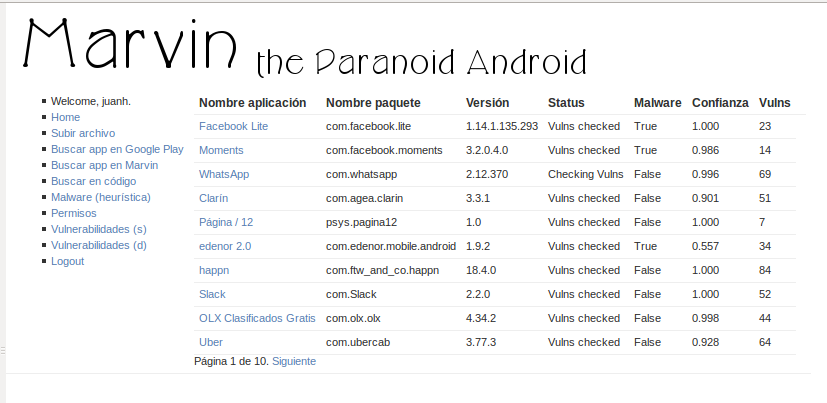
\includegraphics[width=\textwidth]{graphics/marvin_main.png}
\caption{Marvin Home Screen}
\end{figure}
Marvin's Home Screen is split in two: to the left is the actions menu (which is always there) and to the right is a list of the last 10 uploaded apps. From left to right the list shows:

\begin{itemize}
\item The app's ``fantasy'' name.
\item The app's package name, which functions as its identifier in the Google Play Store.
\item The app's version number.
\item App's process status (usually 'queued', 'checking vulns' or 'vulns checked').
\item Whether the permissions heuristics determined that the app could be malware and with how much confidence.
\item The number of potential vulnerabilities found for the app.
\end{itemize}
Clicking on the fantasy name brings us to the app's Information page. See Section \ref{appinfo}.
\section{Actions menu}
\begin{figure}[H]
\begin{center}
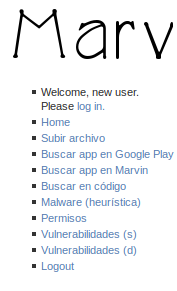
\includegraphics[width=.4\textwidth]{graphics/marvin_panel.png}
\caption{Actions menu}
\end{center}
\end{figure}
Actions menu is where all of Marvin's activities are started. From top to bottom, these are:
\begin{itemize}
\item Login (some actions require being logged in)
\item Go to Home page.
\item Upload a file: It allows uploading of \texttt{.apk} files.
\item Search the Play Store: It allows searching and downloading of apps from the Google Play Store.
\item Search Marvin: You can search for apps alredy uploaded, by app name or by package name.
\item Search in the code: You can search the code for specific strings, such as library, class, or method names.
\item Malware (heuristics): It gives an ordered list of apps for which the permissions list gave the impression that it could be malware, ordered by how strong the impression was.
\item Permissions: Gives a list of the permissions Marvin found, together with the number of apps requesting each one.
\item Vulnerabilities(s): Gives a list of the vulnerabilities that Marvin seeks via static analysis, ordered by the number of found instances.
\item Vulnerabilities(d): Gives a list of the vulnerabilities that Marvin seeks via dynamic analysis, ordered by the number of found instances.
\item Logout 
\end{itemize}

\subsection{App information}\label{appinfo}
In any application list, clicking the name of the app brings us to the app information page. This page has three sections:
\begin{itemize}
\item Metadata and repository access
\item Heuristics, permissions and components
\item Vulnerabilities
\end{itemize}
\begin{figure}[H]
\begin{center}
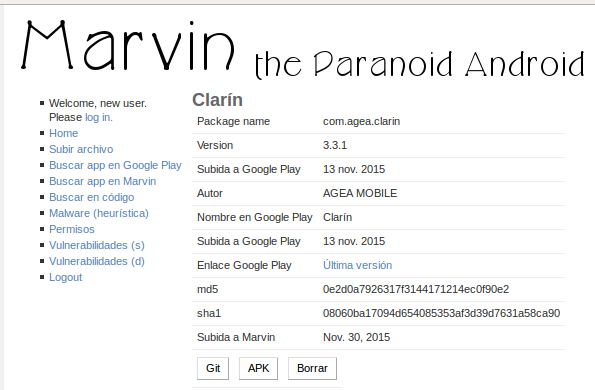
\includegraphics[width=.8\textwidth]{graphics/marvin_app1.png}
\caption{Metadata and repository access}
\end{center}
\end{figure}

In the metadata and repository access section we can see data such as the date an app was uploaded to Google Play, its version number, or the app file checksums, as well as access the Git repository for the app, the APK file itself, or the Google Play page for it (although in this case we are brought to the page for the last uploaded version). We can also delete an app from Marvin here.

\begin{figure}[H]
\begin{center}
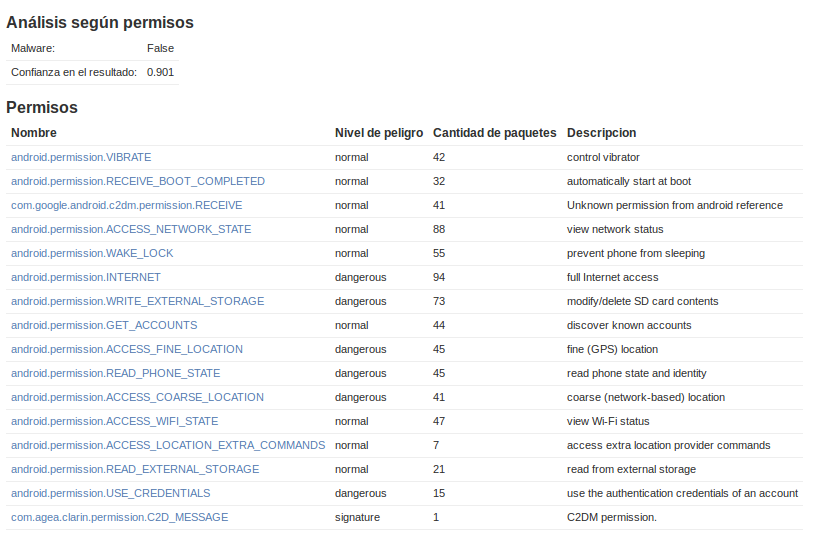
\includegraphics[width=\textwidth]{graphics/marvin_app2.png}
\caption{Heuristics and permissions}
\end{center}
\end{figure}

The heuristics and permissions section shows the result of the Bayesian analysis of the permissions requested by the app, as well as the list of said permissions. The permissions list gives for each permission its name, its danger level, the number of packages that request it, and a succint description of what granting it implies. Clicking on a permission name brings us to a page with stats for the permission (see Section \ref{permissions}).
\begin{figure}[H]
\begin{center}
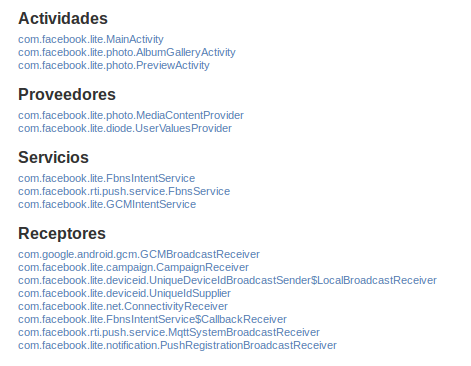
\includegraphics[width=.8\textwidth]{graphics/marvin_app3.png}
\caption{Components section}
\end{center}
\end{figure}

The components section shows us the activities, providers, services and event receivers of an application. If the decompilation process has finished, clicking on any of these will bring up a new browser tab with the GitLab page for its source code. 
 \begin{figure}[H]
\begin{center}
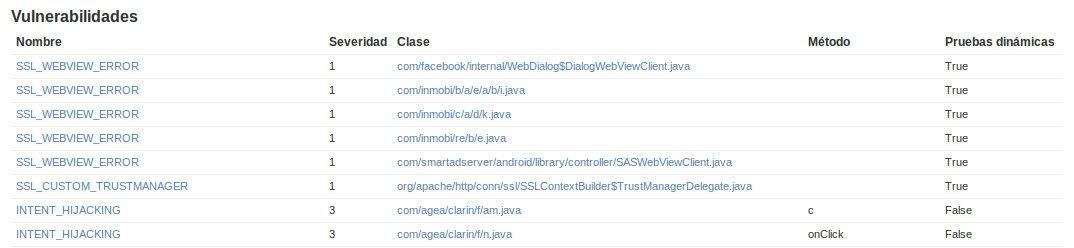
\includegraphics[width=\textwidth]{graphics/marvin_app4.png}
\caption{Vulnerabilities}
\end{center}
\end{figure}

The Vulnerabilities section shows us a list of the vulnerabilities found by \texttt{marvin-static-analyzer}; for each vulnerability found, we can see its type, its severity, the class where it was found, the method if applicable, and whether it can be verified by dynamic analysis. Clicking on the vulnerability type gives us information about the type, while clicking on the class name brings up a new tab with the GitLab page for its source code.

\subsection{Search the Google Play Store}
Marvin can search and download apps from Google Play Store. For this, select ``Search Google Play'' in the Actions menu, enter the search terms, and press Enter.
\begin{figure}[H]
\begin{center}
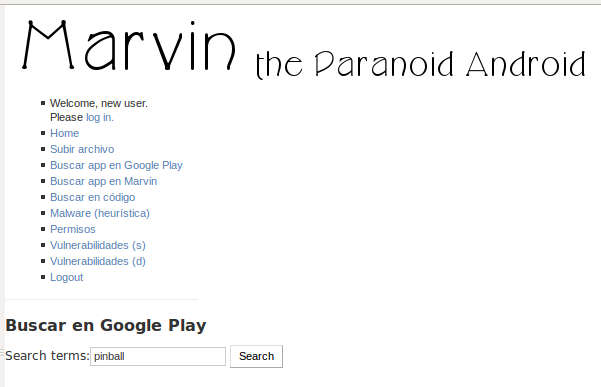
\includegraphics[width=.6\textwidth]{graphics/marvin_gplay.png}
\caption{Google Play Search - Search terms}
\end{center}
\end{figure}

\begin{figure}[H]
\begin{center}
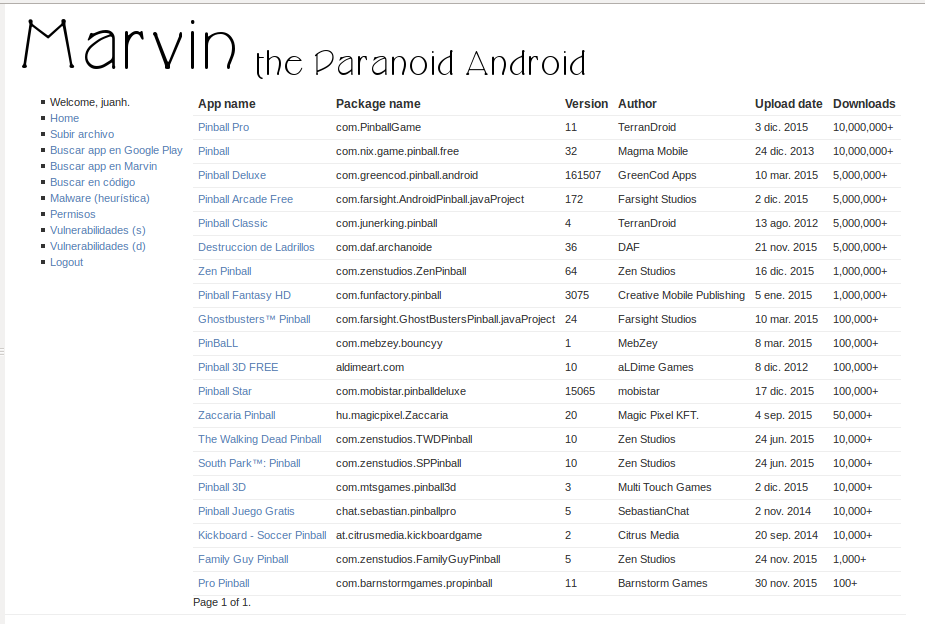
\includegraphics[width=.8\textwidth]{graphics/marvin_gplay2.png}
\caption{Google Play Search - Results} \label{gplay2}
\end{center}
\end{figure}
The results page is as seen in Figure \ref{gplay2}: it has some basic data for each app, plus the upload date to Google Play and the number of downloads. If we click on any of the apps, we are brought to a page like the one in Figure \ref{gplay3}, where some more information is shown such as the description and the permissions it requests, and finally there's a button for downloading the app to Marvin and starting analysis.

The analysis: First the app is decompiled, then static analysis is performed on it. Nevertheless, uploading of sources to the repositories takes a long time, so it's common for the results of static analysis (and with them links to the sources in the App info page) to be there before the Gitlab page for them is ready.


\begin{figure}[H]
\begin{center}
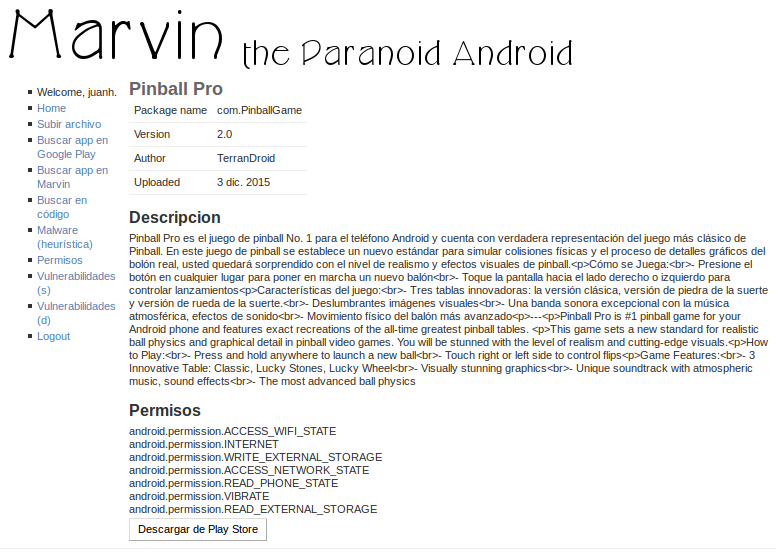
\includegraphics[width=.8\textwidth]{graphics/marvin_gplay3.png}
\caption{Google Play Search- Description} \label{gplay3}
\end{center}
\end{figure}

\subsection{Code Search}
The ``Search Code'' option allows us to search for specific strings in the code, for example to search for use of specific libraries or Android services. After writing the search terms and pressing Enter, the results will show as in Figure \ref{ssource2}: for each match, there's the class name, the app it belongs to, and the length of the source file. Clicking on the file name brings us to the GitLab page for its source code.

\begin{figure}[H]
\begin{center}
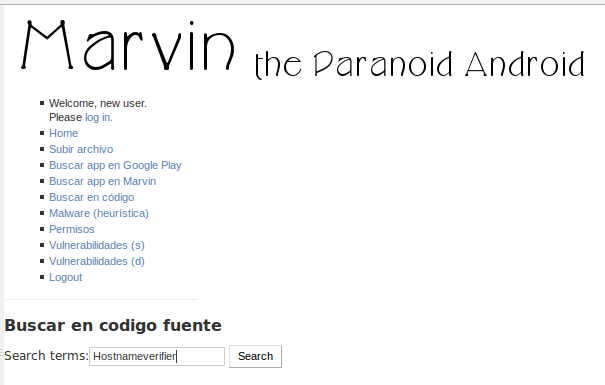
\includegraphics[width=.7\textwidth]{graphics/marvin_searchsource1.png}
\caption{Code search} \label{ssource1}
\end{center}
\end{figure}

\begin{figure}[H]
\begin{center}
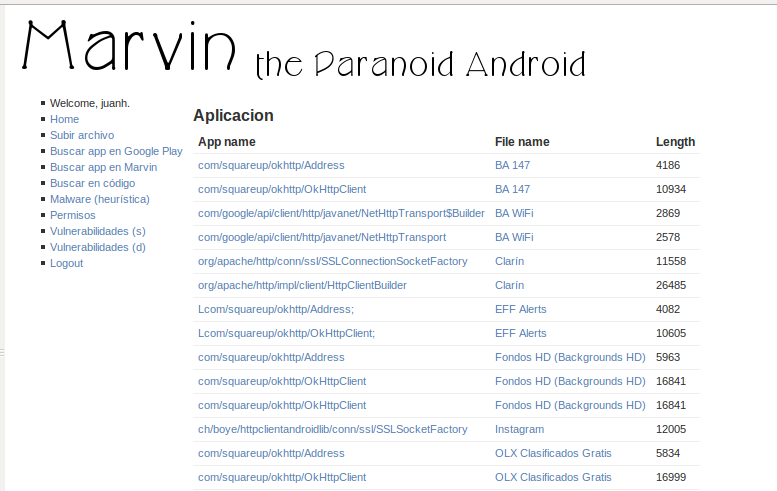
\includegraphics[width=\textwidth]{graphics/marvin_searchsource2.png}
\caption{Code search - Results} \label{ssource2}
\end{center}
\end{figure}

\subsection{Malware (heuristics)}
This option shows an ordered list of the apps that according to the heuristics are most likely to be malware. Together with version information, we can see a score that marks the confidence in the result, and the amount of vulnerabilities Marvin found in the app.
\begin{figure}[H]
\begin{center}
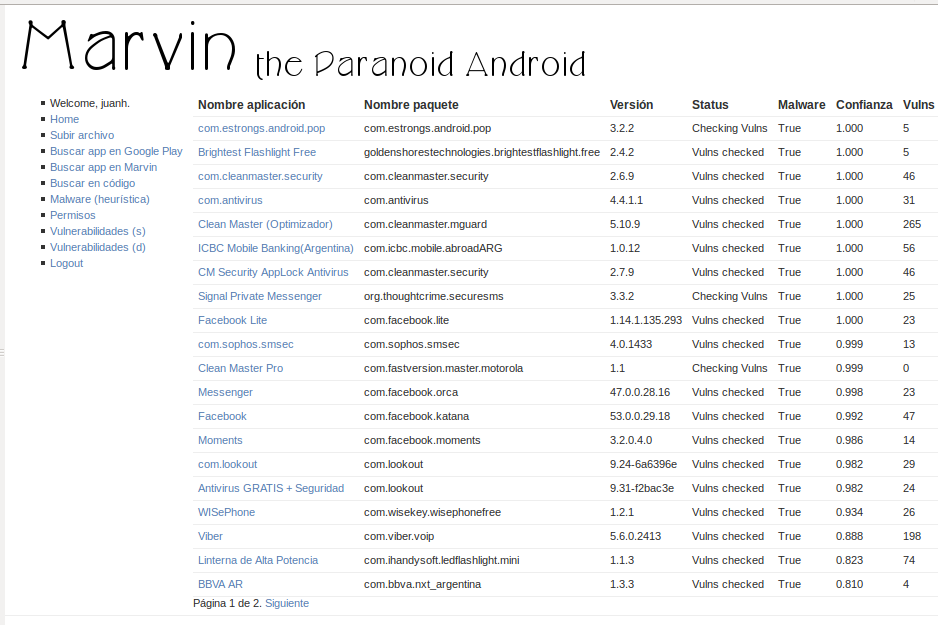
\includegraphics[width=\textwidth]{graphics/marvin_bayesboys.png}
\caption{Malware according to the permissions heuristics} \label{bayes}
\end{center}
\end{figure}
\subsection{Permissions}\label{permissions}
This option shows us the permissions seen by Marvin among all the applications, together with their respective descriptions, danger levels and the number of applications that request them (see Figure \ref{perms}). Clicking on a permission's name brings us to a page with the list of applications that request it (see Figure \ref{appsbyperm}).
\begin{figure}[H]
\begin{center}
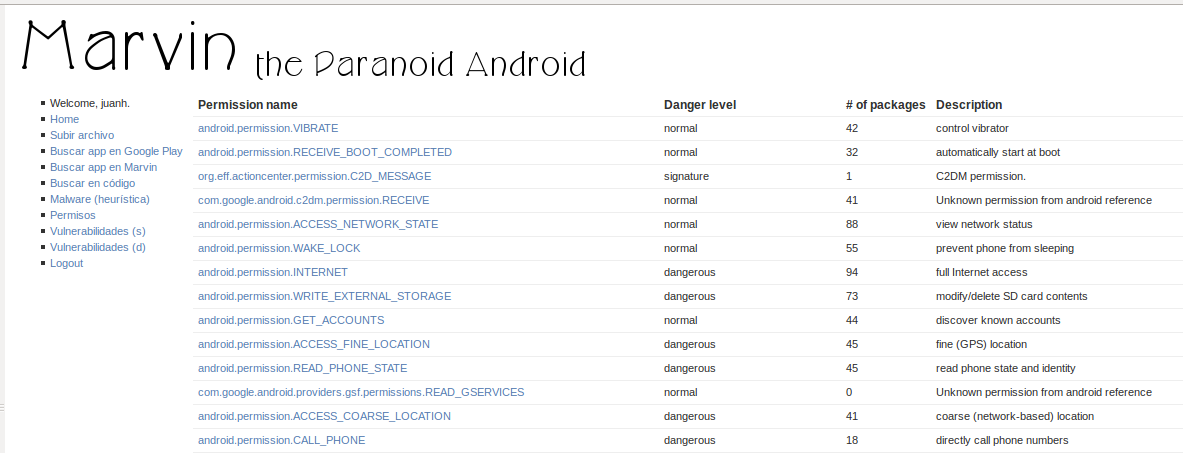
\includegraphics[width=\textwidth]{graphics/marvin_permissions.png}
\caption{Permissions seen by Marvin} \label{perms}
\end{center}
\end{figure}

\begin{figure}[H]
\begin{center}
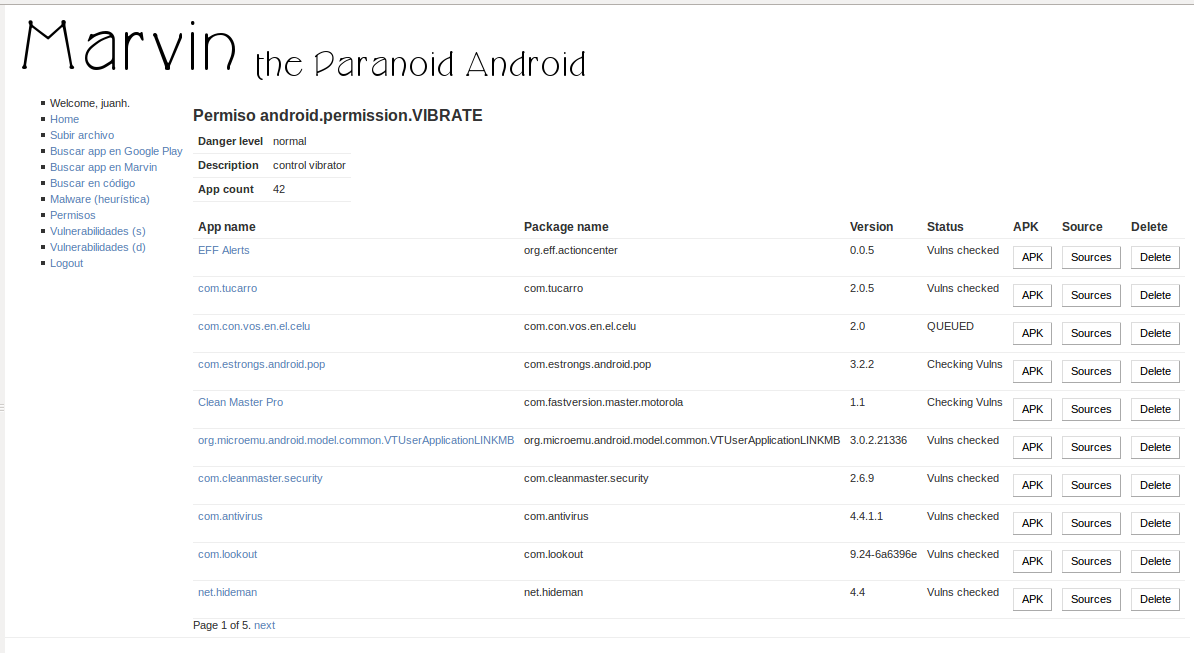
\includegraphics[width=\textwidth]{graphics/marvin_permissions2.png}
\caption{Apps requesting a given permission} \label{appsbyperm}
\end{center}
\end{figure}

\subsection{Vulnerabilities}

In this section we can see the vulnerability types that Marvin knows about and can find, statically as well as dynamically. Some of the vulnerabilities it finds via static analysis can be verified by dynamic analysis, and some are directly searched for via dynamic analysis. For each vulnerability type, Marvin shows a list ordered by the number of applications where it is found (see Figure \ref{vulns}). If we click on the vulnerability type name, Marvin shows us the list of apps where it was found (see Figure \ref{vulns2}).

\begin{figure}[H]
\begin{center}
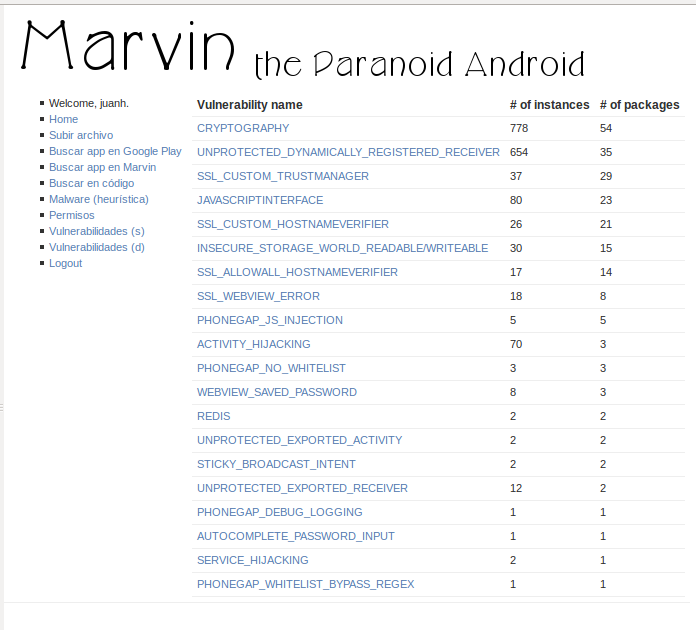
\includegraphics[width=\textwidth]{graphics/marvin_vulns.png}
\caption{List of vulnerability types known to Marvin} \label{vulns}
\end{center}
\end{figure}

\begin{figure}[H]
\begin{center}
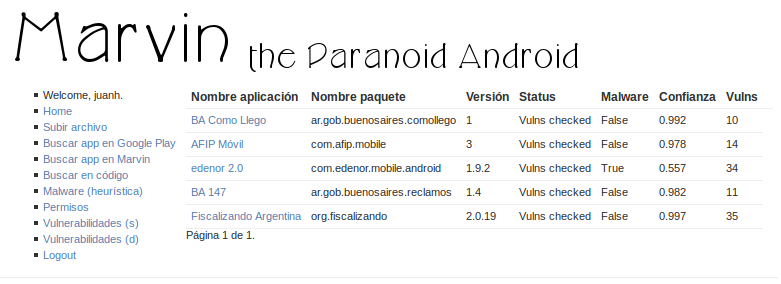
\includegraphics[width=\textwidth]{graphics/marvin_vulns2.png}
\caption{List of apps with a given vulnerability} \label{vulns2}
\end{center}
\end{figure}

\section{Administration}
In the Administration section we can manage user accounts for Marvin and the access data for the Play Store. This section can be accessed at \texttt{http://url\_marvin/admin}.

\begin{figure}[H]
\begin{center}
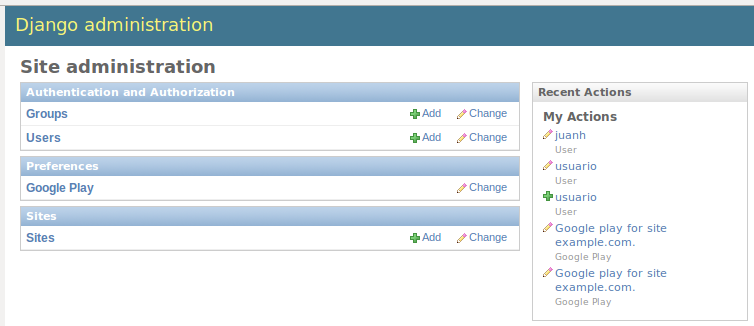
\includegraphics[width=\textwidth]{graphics/marvin1.png}
\caption{Administration} \label{admin}
\end{center}
\end{figure}
\subsection{User accounts}
Clicking 'Users' we enter the Marvin user administration proper:
\begin{figure}[H]
\begin{center}
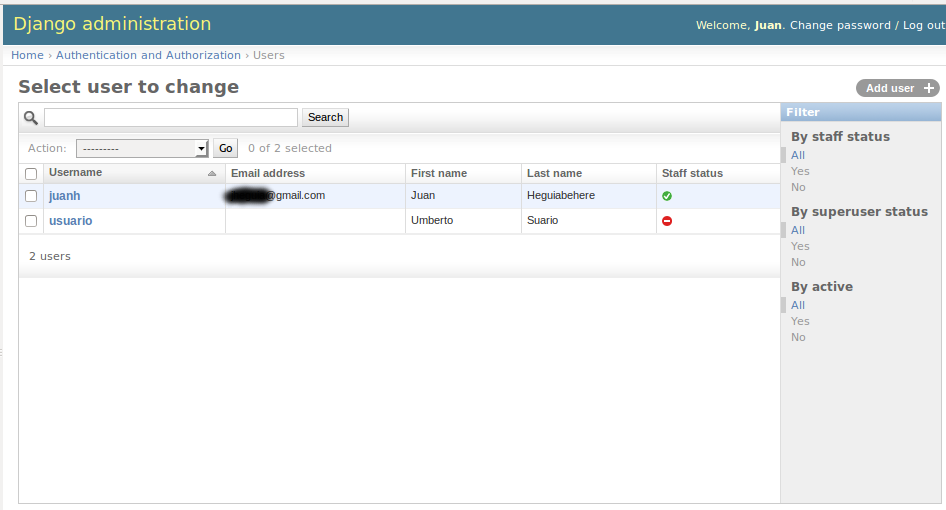
\includegraphics[width=\textwidth]{graphics/marvin2.png}
\caption{Administration - Users} \label{adminus}
\end{center}
\end{figure}

In this section we can create, update and delete Marvin user accounts (so far all users have the same access to all data, but still we want to make sure only logged in users can do some things). User management is straightforward:

\begin{figure}[H]
\begin{center}
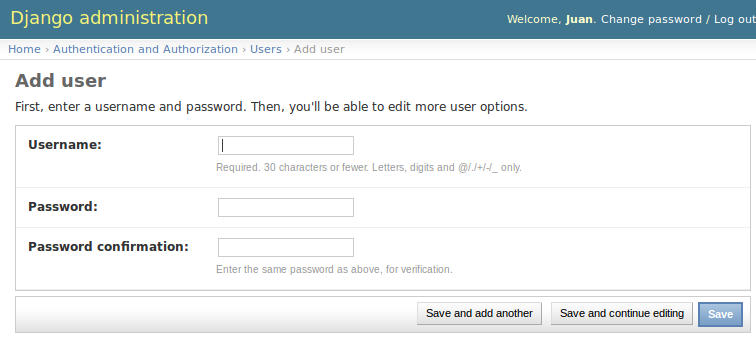
\includegraphics[width=\textwidth]{graphics/marvin4.png}
\caption{Administration - New User} \label{altaus}
\end{center}
\end{figure}
\subsection{Google Play account}
\begin{figure}[H]
\begin{center}
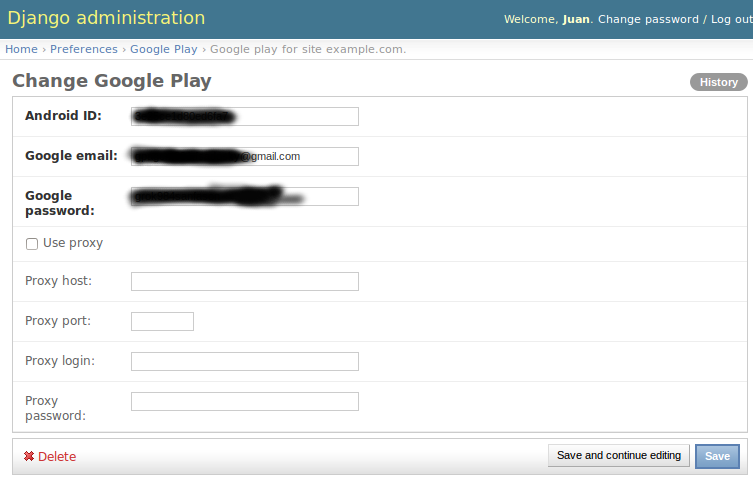
\includegraphics[width=\textwidth]{graphics/marvin3.png}
\caption{Administration - Google Play account} \label{googleplay_acct}
\end{center}
\end{figure}
The Google Play section lets us input the credentials of a Gmail account to access the Play Store. Of course, such account should be 'checked in' the Play Store. This can be an account used on a phone, or (better) one checked in via the \texttt{android-checkin} program, written by Nicolas Viennot: \texttt{https://github.com/nviennot/android-checkin}

\end{document}
